% 请在下方的大括号相应位置填写正确的节标题和标签,以及作者姓名
\section{态密度基础}\label{sec:态密度基础}
\sectionAuthor{Jiaqi Z.}

% 请在下方的item内填写本节知识点
\begin{Abstract}
    \item 态密度(DOS)的概念
    \item 分波态密度(PDOS)的概念
    \item DOS图与PDOS图的简要分析方法
\end{Abstract}

在本章我们将要讨论态密度(Density of State, DOS)的计算。从物理实质上来说,态密度和能带所包含的信息是大致相同的。例如,通过态密度和能带我们都可以知道材料带隙值的大小,判断导电性。但相比于能带,态密度还具有如下不同:

\begin{itemize}
    \item 对于超胞(通常还包括掺杂)等情况,能带结构会变得复杂,通常需要配合反折叠技术进行解释;而态密度对于超胞则是\emph{成比例缩放},因此会更加直观;
    \item 态密度相比于能带,可以计算分波态密度(Projected Density of State, PDOS)。利用PDOS,可以看到原子轨道(如O的2p轨道、Ti的3d轨道等)对态密度的贡献,从而可以进一步分析其物理机理;
    \item DOS图在绘制时忽略了波矢$k$信息,因此根据态密度无法分析带隙的类型是直接带隙或间接带隙。因此对于动量相关的信息,只能通过能带进行分析\footnote{进一步地,能带可以根据价带顶和导带底的能量对$k$的导数得到有效质量,DOS图就无法得到这一结论。}。
\end{itemize}

因此,在本章,我们将讨论如何使用VASP计算态密度,包括总态密度与分波态密度,还会包括考虑自旋极化的态密度绘制。

\subsection{态密度概念}\label{subsec:态密度基础-态密度概念}

我们并不会在这里详细说明态密度与能带的详细推导方法(可以参考相关的物理教材)。简单来说,在固体中由于电子的能级非常密集,为\emph{准连续分布},因此像原子那样标定每个能级是没有意义的。参考对应的概念,考虑能量在$E\sim E+\Delta E$之间的电子态数目,若电子态数目由为$\Delta Z$,则态密度定义为

\begin{equation*}
    N(E)=\lim\limits\frac{\Delta Z}{\Delta E}
\end{equation*}

对于已知能带而言,即已知$E(k)$关系,通过推导(参考黄昆著《固体物理学》)可以知道其态密度可以表示为

\begin{equation*}
    N(E)=\frac{V}{(2\pi)^3}\int\frac{\dd{S}}{\abs{\nabla_kE}}
\end{equation*}

除此之外,在考虑电子态的时候,如果仅考虑某个原子轨道的电子对能带的贡献,则所绘制的\emph{仅考虑对应轨道电子}的态密度称为\emph{投影态密度}(Projected Density of States, PDOS)。

\subsection{简要分析态密度和投影态密度}\label{subsec:态密度基础-简要分析态密度和投影态密度}

与能带类似,态密度也可以用来判断材料的带隙(但不能判断带隙类型为直接带隙还是间接带隙)。例如,在后面我们将会计算得到Si的态密度如图\ref{fig:态密度基础-Si态密度}所示。可以发现,Si的带隙大约为0.7 eV。

\begin{figure}
    \centering
    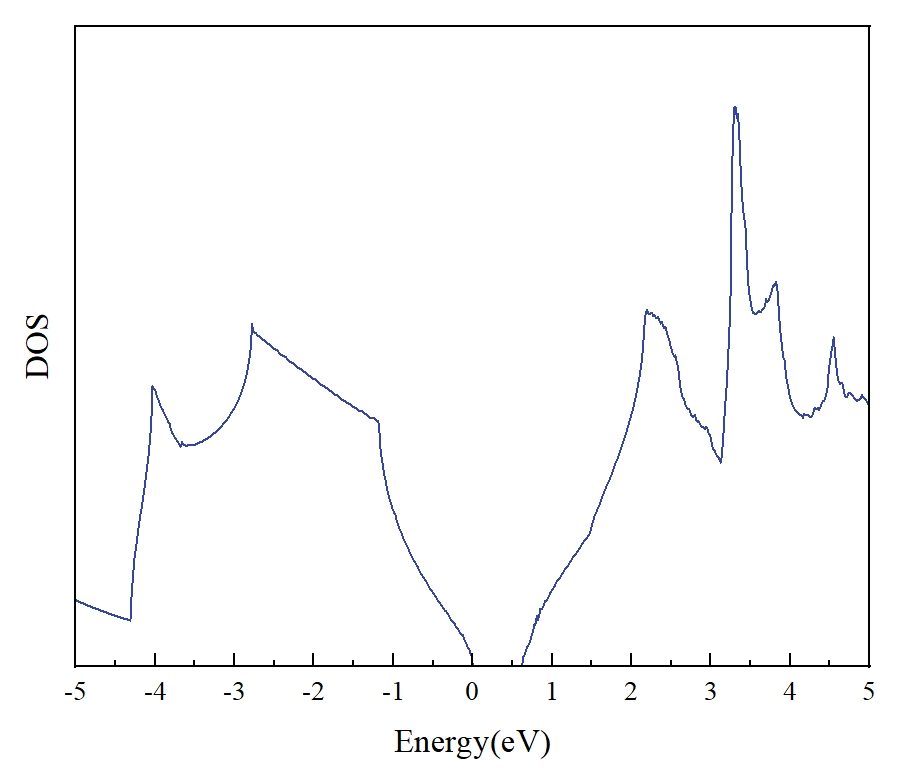
\includegraphics[width=1\linewidth]{VASP计算/态密度计算/态密度基础/fig/Si态密度.png}
    \caption{Si态密度}
    \label{fig:态密度基础-Si态密度}
\end{figure}

再比如,对于PDOS而言,我们可以通过态密度的重叠情况判断原子之间的杂化成键。例如,图\ref{fig:态密度基础-PDOS例子}中计算了Li吸附在不同\ch{TiS2}下的态密度,可以发现Li和Ti,Li和S之间存在着轨道重叠,表明两个原子的电子处在同一个电子态,即发生了\emph{轨道杂化}\footnote{参考文献:Tian, R. et al. Point defects-induced adsorption and diffusion of lithium on monolayer titanium disulfide: A first-principles study. Applied Surface Science 553, 149448 (2021).}。

\begin{figure}
    \centering
    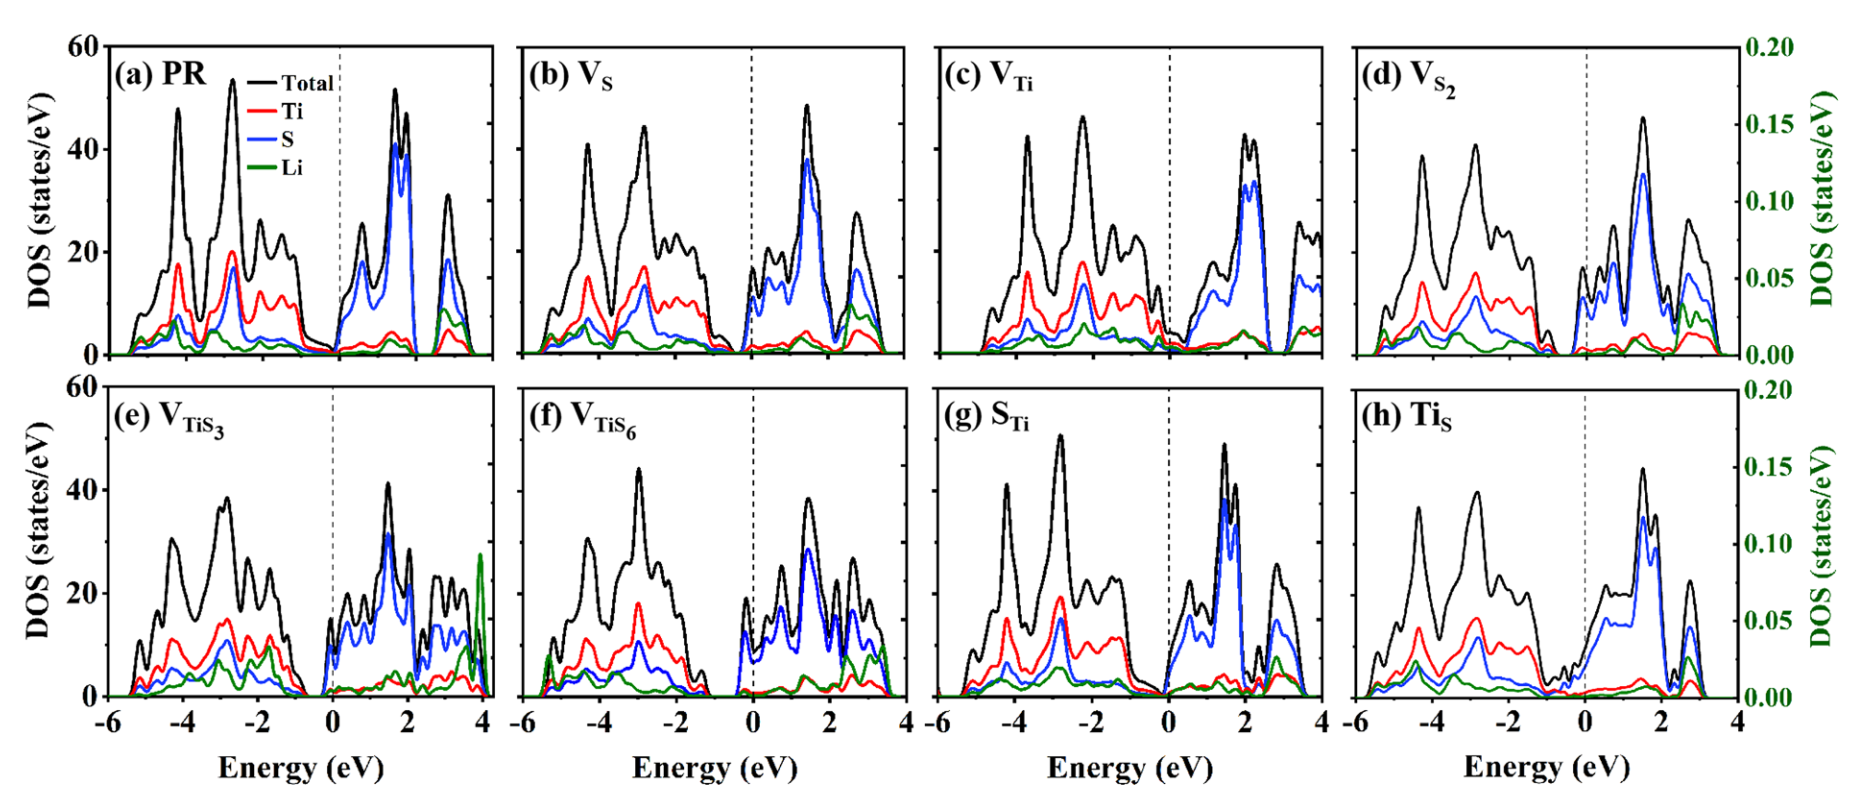
\includegraphics[width=1\linewidth]{VASP计算/态密度计算/态密度基础/fig/PDOS例子}
    \caption{PDOS例子}
    \label{fig:态密度基础-PDOS例子}
\end{figure}

% \subsubsection{小小节标题}

% \subsection{小节标题}\label{subsec:节标题-小节标题}


% \subsection{错误处理}\label{subsec:节标题-错误处理}
% % 请在本节列出可能遇见的错误与解决方法

% \subsubsection{错误1}

% \subsubsection{错误2}

% \subsubsection{错误3}